\chapter{Superfici Intelligenti Riconfigurabili}
In questo ultimo capitolo cercheremo di analizzare, almeno superficialmente, le RIS (Reconfigurable Intelligent Surface), ovvero delle strutture planari con N elementi riflettenti posti tra loro a distanza minore della lunghezza d'onda:
\begin{center}
    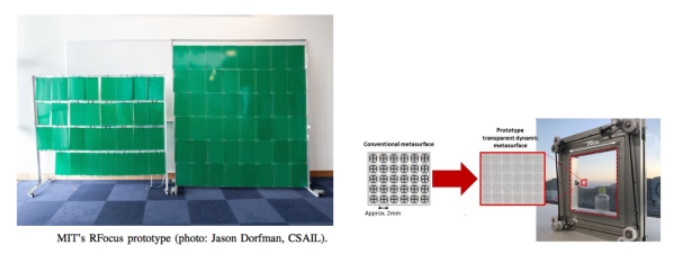
\includegraphics[width=0.8\textwidth]{Images/RIS.png}
\end{center}
Ogni elemento può riflettere un segnale elettromagnetico che arriva su di sè, con un Coefficiente di Riflessione $\Gamma_n$.\\ \\
Una RIS è una struttura quasi-passiva dato che non usa amplificatori ed ha un hardware molto semplice, e per questo a un consumo energetico inferiore ad antenne tradizionali.
Possono essere usate per:
\begin{itemize}
    \item Creare nuovi canali
    \item Cancellare segnali interferenti
\end{itemize}

\section{Ris: Uplink}
Supponendo di essere nel seguente caso:
\begin{itemize}
    \item K utenti serviti da una BS con L antenne
    \item $\vc{h}_{k,RIS}$ è il canale N X 1 tra l'utente k e gli N elementi della RIS
    \item $\vc{G}_{RIS}$ è il canale L X N tra gli N elementi della RIS e la BS
\end{itemize}
Alla RIS arriverà il seguente segnale:
\begin{equation*}
    \vc{r} = \sum_{k=1}^K \sqrt{p_k} \vc{h}_{k,RIS} s_k = \sum_{k=1}^K \sqrt{p_k} \begin{pmatrix} 
    \vc{h}_{k,RIS} (1) \\
    \vc{h}_{k,RIS} (2) \\
    \vdots \\
    \vc{h}_{k,RIS} (N) \\
    \end{pmatrix}
    s_k
\end{equation*}
A questo punto la RIS trasmette il segnale tramite la matrice diagonale $\Gamma$, che ha come diagonali i coefficienti di riflessione:
\begin{equation*}
    \begin{pmatrix}
    \Gamma_1 & 0 & \dots & \dots & 0 \\
    0 & \Gamma_2 & 0 & \dots & 0 \\
    \vdots & \vdots & \vdots & & \vdots \\
    0 & 0 & 0 & \dots & \Gamma_N
    \end{pmatrix}
\end{equation*}
Alla BS il segnale ricevuto verrà filtrato con $\vc{c}_m$ per demodulare il simbolo dell'utente m;
\begin{equation*}
    y = \vc{c}_m^H \vc{G}_{RIS} \vc{\Gamma} \vc{r} = \sum_{k=1}^K \sqrt{p_k} \vc{c}_m^H \vc{G}_{RIS} \vc{\Gamma} \vc{h}_{k,RIS} s_k + n
\end{equation*}
Il SINR dell'utente m quindi sarà:
\begin{equation*}
    SINR_m = \frac{p_m |\vc{c}_m^H \vc{G}_{RIS} \vc{\Gamma} \vc{h}_{m,RIS}|^2}{\sigma^2 + \sum_{k \cancel{\in}} p_k |\vc{c}_m^H \vc{G}_{RIS} \vc{\Gamma} \vc{h}_{k,RIS}|^2}
\end{equation*}
Ora se definiamo il Canale Equivalente $\vc{v}_m = \vc{G}_{RIS} \vc{\Gamma} \vc{h}_{m,RIS}$ possiamo riusarla teoria del Filtraggio Adattato.


\section{RIS: Downlink}
Nel downlink possiamo procedere in modo analogo definendo:
\begin{itemize}
    \item $\vc{H}_{RIS}$ il canale tra la BS e la RIS
    \item $\vc{g}_{m,RIS}$ il canale tra la RIS e l'utente m
    \item $\vc{q}_m$ il vettore di Beamforming dell'utente m
\end{itemize}
quindi il segnale che la RIS riceverà sarà:
\begin{equation*}
    \vc{r} = \vc{H}_{RIS} \sum_{k=1}^K \sqrt{p_k} s_k \vc{q}_k
\end{equation*}
A questo punto la RIS riflette il segnale tramite la matrice $\vc{\Gamma}$:
\begin{equation*}
    \begin{pmatrix}
    \Gamma_1 & 0 & \dots & \dots & 0 \\
    0 & \Gamma_2 & 0 & \dots & 0 \\
    \vdots & \vdots & \vdots & & \vdots \\
    0 & 0 & 0 & \dots & \Gamma_N
    \end{pmatrix}
\end{equation*}
Il segnale ricevuto dall'utente m sarà:
\begin{equation*}
    y = \vc{g}_{m,RIS}^H \vc{\Gamma} \vc{r} = \sum_{k=1}^K \sqrt{p_k} \vc{g}_{m,RIS}^H \vc{\Gamma} \vc{H}_{RIS}\vc{q}_k s_k + n
\end{equation*} 
Il SINR dell'utente m sarà quindi:
\begin{equation*}
    SINR_m = \frac{p_m |\vc{g}_{m,RIS}^H  \vc{H}_{RIS} \vc{\Gamma} \vc{q}_{m}|^2}{\sigma^2 + \sum_{l \neq k} p_k |\vc{g}_{m,RIS}^H \vc{H}_{RIS} \vc{\Gamma} \vc{q}_{k}|^2}
\end{equation*}
E definendo il vettore di canale equivalente:
\begin{equation*}
    \vc{u}_m^H = \vc{g}_{m,RIS}^H \vc{H}_{RIS} \vc{\Gamma} 
\end{equation*}
possiamo riusare la teoria del Filtro Adattato, scegliendo $\vc{q}_m$.


\section{Allocazione della Matrice Gamma}
Consideriamo un Downlink in un Sistema Singolo Utente e definiamo:
\begin{equation*}
    \vc{H}\vc{q} = \vc{q}_{eq}
\end{equation*}
Ora calcoliamo l'SNR:
\begin{equation*}
    SNR = \frac{p|\vc{g}^H \vc{\Gamma} \vc{H} \vc{q}|^2}{\sigma^2} = \frac{p|\vc{g}^H \vc{\Gamma} \vc{q}_{eq}|^2}{\sigma^2} = \frac{p}{\sigma^2} \left|\sum_{n=1}^N \Gamma_n g_n^* h_n\right|^2 
\end{equation*}
Applicando la disuguaglianza triangolare otteniamo:
\begin{equation*}
    SNR \leq \frac{p}{\sigma^2} \left(\sum_{n=1}^N |\Gamma_n| |g_n| |h_n|\right)^2 \leq \frac{p}{\sigma^2} \left(\sum_{n=1}^N |g_n| |h_n|\right)^2 
\end{equation*}
A questo punto l'uguaglianza si otterrà per ogni n scegliendo:
\begin{itemize}
\item $\phase{\Gamma_n} = - \phase{g_n^*} h_n$
\item $|\Gamma_n| = 1 $
\end{itemize}

\subsection{Caso Multi-Utente}
Nel caso multi-utente l'ottimizzazione di $\vc{\Gamma}$ è più complicata perchè non è possibile scegliere $\vc{\Gamma}$ in modo da compensare le fasi dei canali di tutti gli utenti.